\documentclass[border=4pt]{standalone}
\usepackage{tikz}

\begin{document}
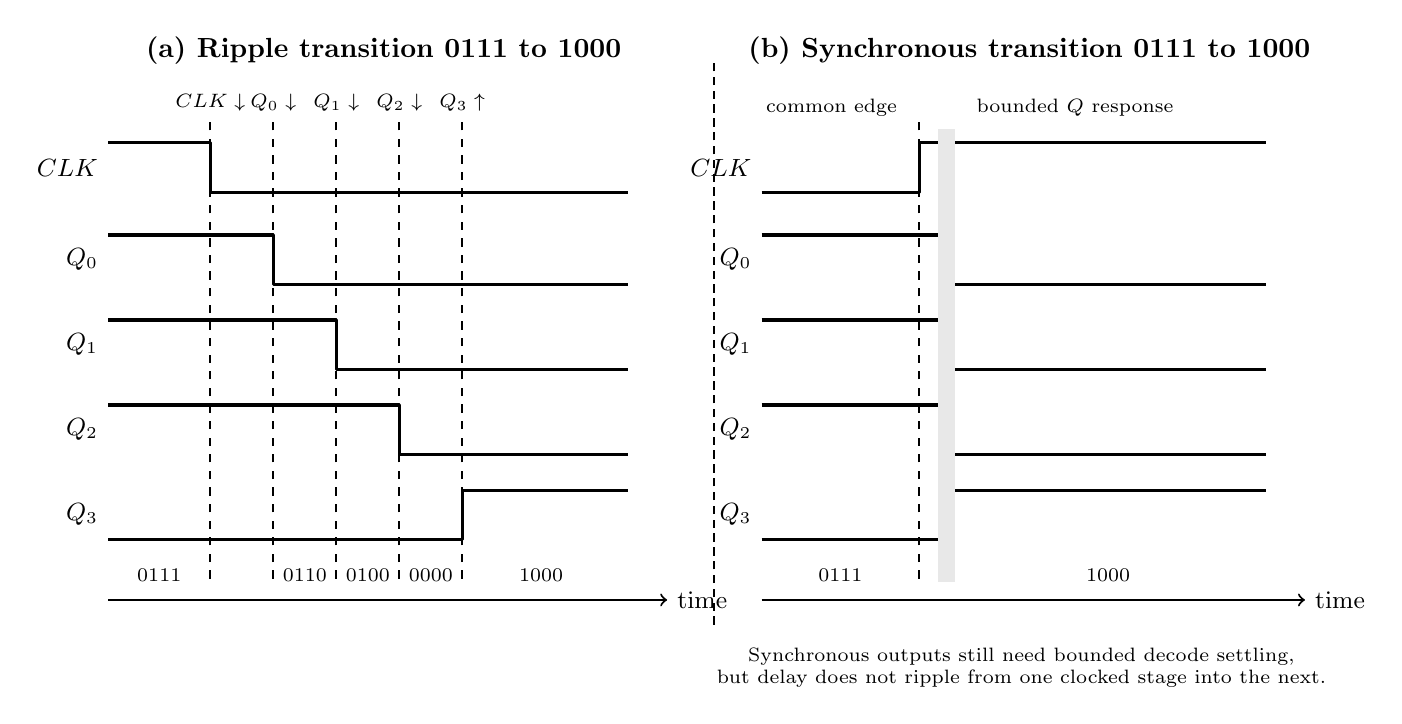
\begin{tikzpicture}[x=1cm,y=0.9cm,font=\small,line width=0.75pt,
  thick/.style={line width=1.15pt,line join=round}]
  \node[font=\bfseries] at (4.2,8.15) {(a) Ripple transition 0111 to 1000};
  \draw[->] (0.7,0.4) -- (7.8,0.4) node[right] {time};
  \foreach \y/\name in {6.5/$CLK$,5.2/$Q_0$,4.0/$Q_1$,2.8/$Q_2$,1.6/$Q_3$}
    \node[left] at (0.7,\y) {\name};
  \draw[thick] (0.7,6.85) -- (2.0,6.85) -- (2.0,6.15) -- (7.3,6.15);
  \draw[thick] (0.7,5.55) -- (2.80,5.55) -- (2.80,4.85) -- (7.3,4.85);
  \draw[thick] (0.7,4.35) -- (3.60,4.35) -- (3.60,3.65) -- (7.3,3.65);
  \draw[thick] (0.7,3.15) -- (4.40,3.15) -- (4.40,2.45) -- (7.3,2.45);
  \draw[thick] (0.7,1.25) -- (5.20,1.25) -- (5.20,1.95) -- (7.3,1.95);
  \foreach \x/\lab in {2.0/$CLK\downarrow$,2.8/$Q_0\downarrow$,3.6/$Q_1\downarrow$,4.4/$Q_2\downarrow$,5.2/$Q_3\uparrow$}
    \draw[dashed] (\x,0.7) -- (\x,7.15) node[above,font=\scriptsize] {\lab};
  \node[font=\scriptsize] at (1.35,0.75) {0111};
  \node[font=\scriptsize] at (3.2,0.75) {0110};
  \node[font=\scriptsize] at (4.0,0.75) {0100};
  \node[font=\scriptsize] at (4.8,0.75) {0000};
  \node[font=\scriptsize] at (6.2,0.75) {1000};

  \draw[densely dashed] (8.4,0.05) -- (8.4,8.0);
  \node[font=\bfseries] at (12.4,8.15) {(b) Synchronous transition 0111 to 1000};
  \draw[->] (9.0,0.4) -- (15.9,0.4) node[right] {time};
  \foreach \y/\name in {6.5/$CLK$,5.2/$Q_0$,4.0/$Q_1$,2.8/$Q_2$,1.6/$Q_3$}
    \node[left] at (9.0,\y) {\name};
  \draw[thick] (9.0,6.15) -- (11.0,6.15) -- (11.0,6.85) -- (15.4,6.85);
  \draw[thick] (9.0,5.55) -- (11.28,5.55) -- (11.28,4.85) -- (15.4,4.85);
  \draw[thick] (9.0,4.35) -- (11.32,4.35) -- (11.32,3.65) -- (15.4,3.65);
  \draw[thick] (9.0,3.15) -- (11.36,3.15) -- (11.36,2.45) -- (15.4,2.45);
  \draw[thick] (9.0,1.25) -- (11.40,1.25) -- (11.40,1.95) -- (15.4,1.95);
  \fill[gray!18] (11.24,0.65) rectangle (11.46,7.05);
  \draw[dashed] (11.0,0.7) -- (11.0,7.15);
  \node[anchor=east,font=\scriptsize] at (10.85,7.35) {common edge};
  \node[anchor=west,font=\scriptsize] at (11.60,7.35) {bounded $Q$ response};
  \node[font=\scriptsize] at (10.0,0.75) {0111};
  \node[font=\scriptsize] at (13.4,0.75) {1000};
  \node[align=center,font=\scriptsize] at (12.3,-0.55)
    {Synchronous outputs still need bounded decode settling,\\
     but delay does not ripple from one clocked stage into the next.};
\end{tikzpicture}
\end{document}
